\section{\gls{mca} ir \LIME \gls{ae} aptikimo metodų sintezė}\label{sec:method}

Autoriaus siūlomas \gls{ae} aptikimo metodas yra apjungti \gls{mca} dimensijų
mažinimo metodą bei \LIME pritaikymą \gls{ae} aptikimui su tam tikromis
modifikacijomis (\ref{sec:method:mods}). Kadangi \gls{mca} ir \LIME atitinka
bazės keitimo \skyrius{sec:literature:defense:basis} ir perkeliamumo
blokavimo \skyrius{sec:literature:defense:blocking} \gls{ae} aptikimo
strategijas, kurios iš aptartų yra perspektyviausios -- jų sinteze tikimasi
gauti dar tikslesnį \gls{ae} aptikimo metodą \zr{fig:original}.

\subsection{\LIME pritaikymo \gls{ae} aptikimui metodo modifikacijos}\label{sec:method:mods}

\noindent
\begin{minipage}{0.45\textwidth}
    \hspace{1cm}
    \ref{sec:literature:defense:ids} skyriuje siūlomas \LIME pritaikymas \gls{ae} aptikimui remiasi svarbiausių (didžiausią įtaką \gls{ml} modelio sprendimų priėmimui turinčių) požymių analize. Svarbiausi požymiai laikomi pirmieji 10 \cite{tcydenovaDetectionAdversarialAttacks2021}. Nors autoriai neaprašo kaip pasirenkama tokia konstanta, akivaizdu, jog ji nėra tinkama visiems atvejams. Pavyzdžiui, turint žymiai daugiau požymių, ši konstanta gali būti per maža. Tokia problema ypač aktuali kai analizuojami kategoriniai požymiai, turintys daug kategorijų (dažniausiai koduojami kaip dvejetainiai vektoriai). Dėl šios priežasties, autoriaus siūlymas yra \enquote{svarbiais} laikyti visus požymius ir mokymo fazės pabaigoje apskaičiuoti šių požymių įtakos \gls{ml} modelio sprendimo priėmimui statistikas (vidurkį ir standartinį nuokrypį). Tuomet aptikimo fazėje naudoti $3 \sigma$ taisyklę \cite{pukelsheimThreeSigmaRule1994}, \ty jei bent vieno požymio įtaka \gls{ml} sprendimo priėmimui nukrypsta per 3 standartinius nuokrypius nuo duotojo požymio vidurkio -- laikyti, jog analizuojama įvestis buvo obfuskuota.
\end{minipage}
\hspace{0.02\textwidth}
\begin{minipage}{0.58\textwidth}
    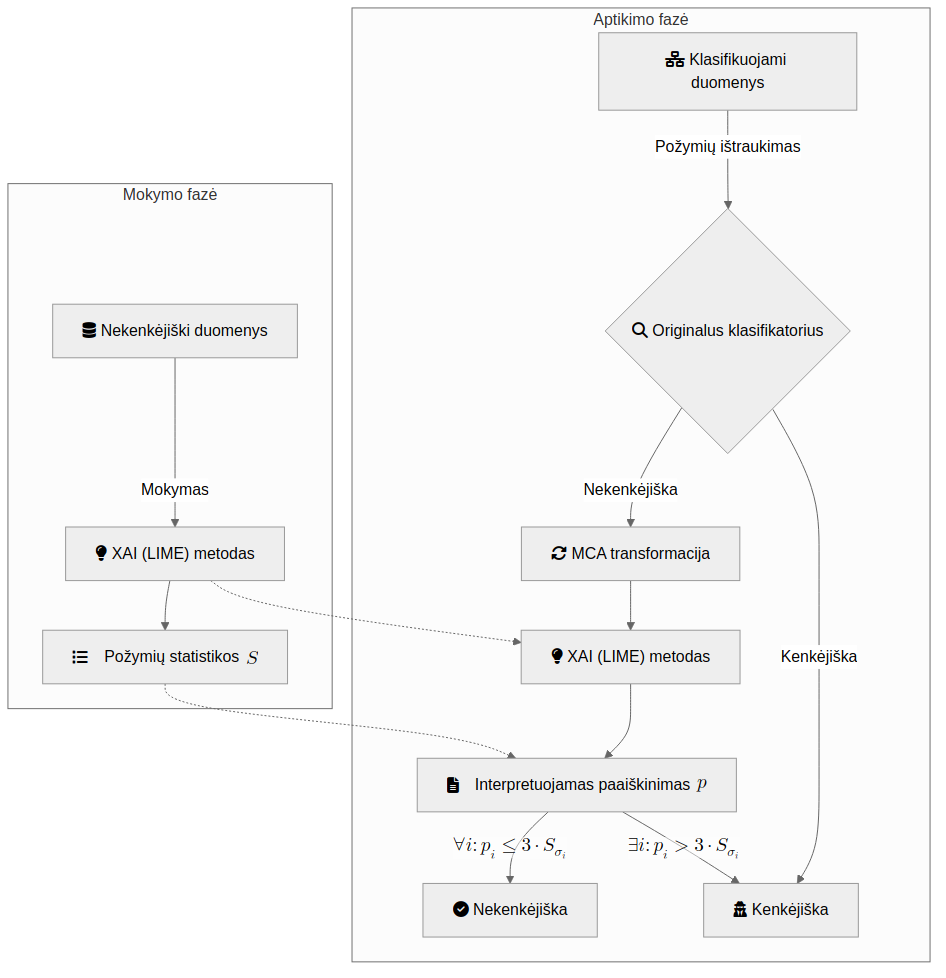
\includegraphics[width=0.95\textwidth]{images/original.png}
    \captionof{figure}{\LIME ir \gls{mca} sintezės \gls{ae} aptikimo metodo iliustracija}
    \label{fig:original}
\end{minipage}

\clearpage
\subsection{\LIME branduolio pločio pasirinkimas}
\LIME branduolio plotį \skyrius{sec:literature:lime} gali padėti nustatyti duomenų vizualizacijos ar kita duomenų analizė. Tai atlikti nėra sudėtinga, kai požymių vektoriaus dimensija nedidelė arba požymiai yra skaitiniai, tačiau turint kategorinius požymius ir atsižvelgiant į jų kodavimą dvejetainiais vektoriais, parinkti tinkamą \LIME branduolio plotį gali būti sudėtinga. Taikant \gls{mca} transformaciją neretai užtenka branduolio pločio vertę parinkti pagal pirmų dviejų komponenčių skalę, kadangi šios dvi komponentės apibūdina didžiausią inerciją. Pavyzdžiui, \ref{fig:scree} pav. vaizduojamu atveju, tinkamos $\omega$ vertės turėtų būti vienetų skalėje (tiksli vertė nustatoma eksperimentiškai).
\begin{figure}[h]
        \centering
        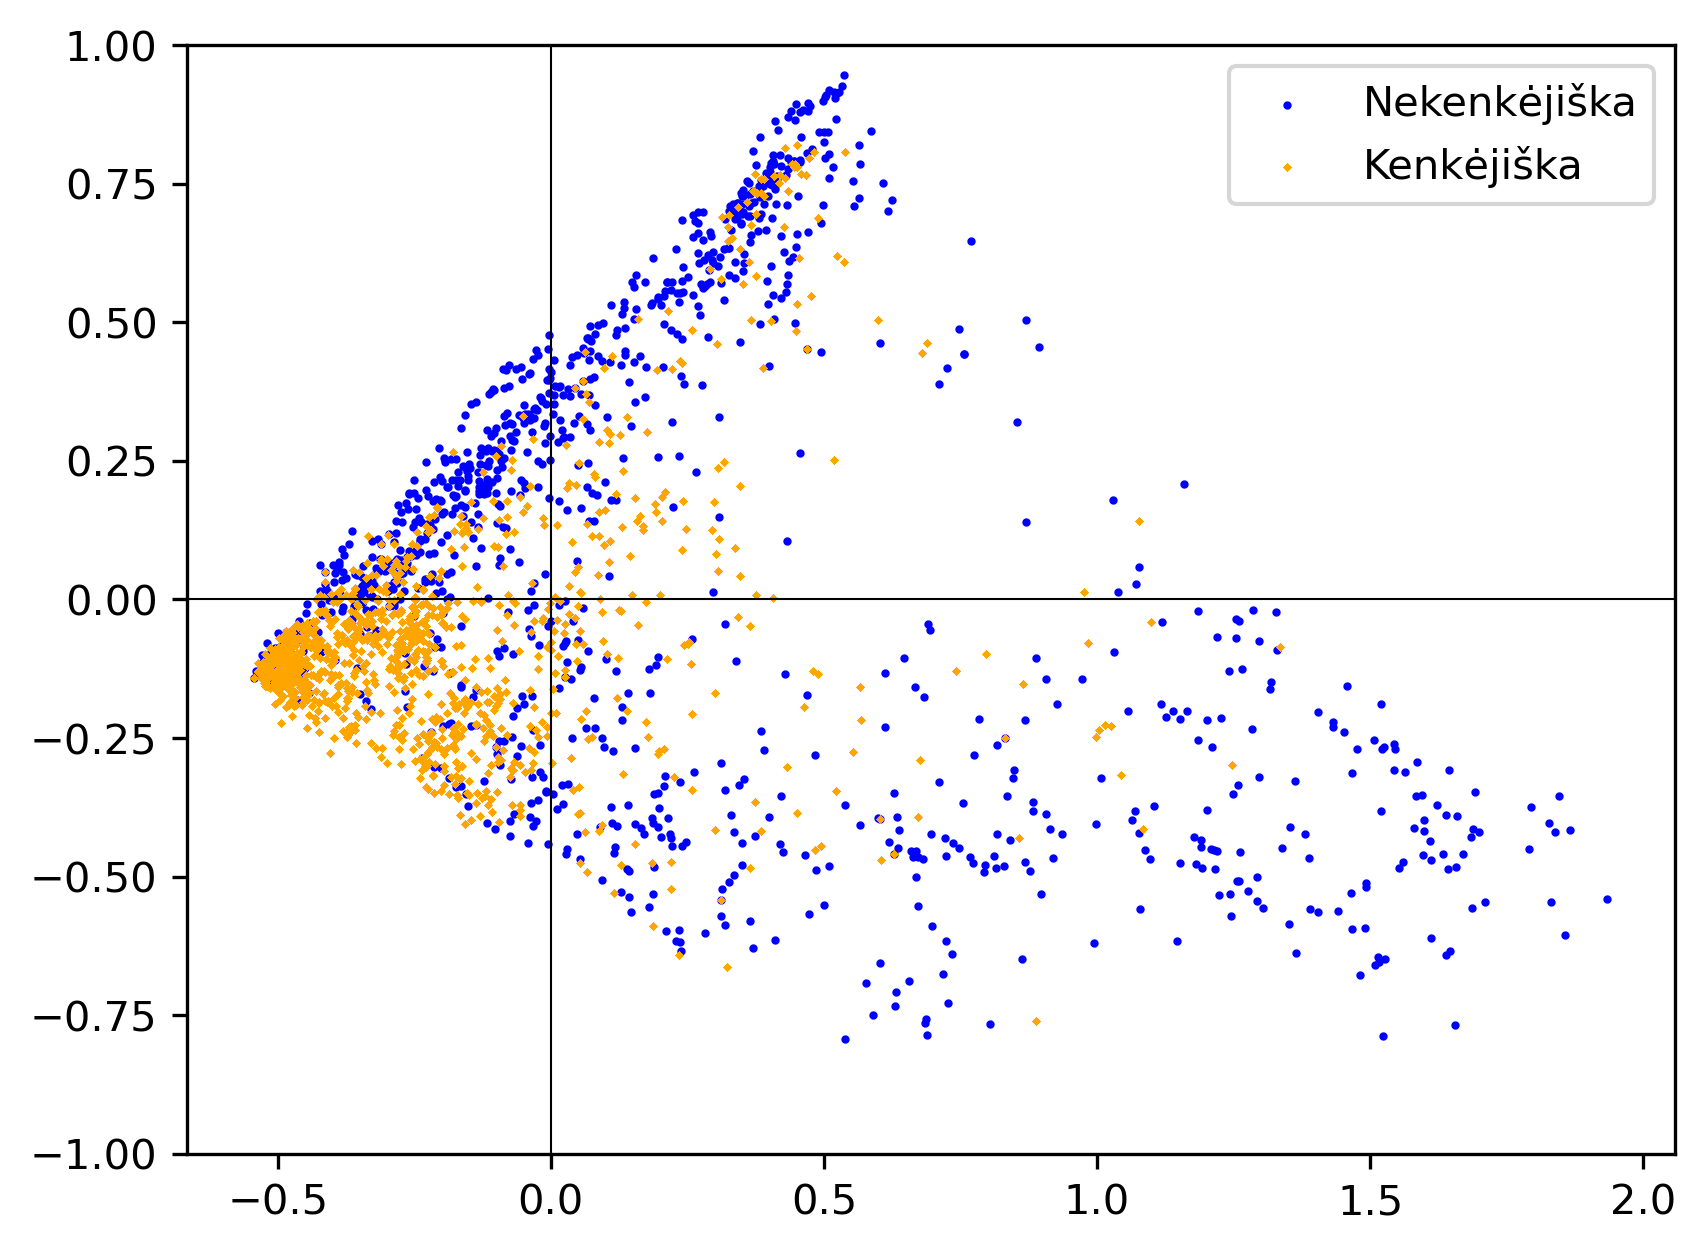
\includegraphics[width=0.55\textwidth]{images/mca_scatter.png}
        \caption{Pirmųjų dviejų \gls{mca} transformacijos komponenčių pavyzdys}
        \label{fig:scree}
\end{figure}

\subsection{Panaudos atvejai}\label{sec:method:usecases}
\begin{enumerate}
    \item {\bfseries \Glsplkam{adversarial} atsparus klasifikatorius.}
     Šiuo atveju naudojamas praplėstas klasifikavimo procesas, visiškai atitinkantis \ref{fig:original}-ią pav. Klasifikatoriaus klasės išlieka tokios pačios. 
    \item {\bfseries \Glsplko{adversarial} indikatorius.} 
    Taip pat naudojamas praplėstas klasifikavimo procesas, tik šiuo atveju, jei originalaus klasifikatoriaus sprendimas buvo klasifikuoti įvestį kaip \textit{nekenkėjišką}, o tolimesnės analizės rezultatas buvo klasifikuoti įvestį kaip \textit{kenkėjišką} -- tuomet įvesčiai priskiriama \textit{obfuskuota} klasė. 
\end{enumerate}

\subsection{Paaiškinamumo aspektas}

Nors \LIME metodas skirtas paaiškinti sudėtingų modelių sprendimus taip, kad žmogus gebėtų juos interpretuoti ir suprasti, autoriaus siūlomas metodas šią savybę praranda. Pagrindinė to priežastis yra tai, jog šiame metode \LIME paaiškina \gls{mca} transformacijos duomenis, kurie savaime nėra interpretuojami. Tuo atveju, kai siūlomas metodas naudojamas kaip \textbf{atakos indikatorius}, tai reiškia, jog šis metodas negali pateikti interpretuojamo paaiškinimo, kodėl tam tikra įvestis yra laikoma obfuskuota.  

% Problem with selecting N components to explain
% Problem with binary feature vectors
% Synthesis of MCA and LIME (original)
% Method flow diagram (adaptation)
% Importance of keeping obfuscation detection hidden (original)